\section*{Reflexión total interna}

\item Verifique o demuestre que:\\
\begin{minipage}[t][4.5cm]{0.65\textwidth}
\begin{enumerate}
	\item Si sobre una lámina de caras paralelas inmersa en un medio de índice de refracción \(n_1\) incide en forma oblicua un rayo este emerge del otro lado con un desplazamiento lateral \(\Delta\).
	Halle una expresión que explicite como su espesor \(d\) e índice de refracción \(n_2\) afectan a \(\Delta\). 
	\item El rayo que se refleja en la primera cara y el que emerge luego de reflejarse en la segunda son paralelos.
\end{enumerate}
Si el medio exterior es único, ¿existe un ángulo de incidencia que produzca reflexión total en la cara inferior?
\end{minipage}
\begin{minipage}[c][0cm][t]{0.33\textwidth}
	\includegraphics[width=\textwidth]{a-000}
\end{minipage}



\item (*)
\begin{minipage}[t][3.5cm]{0.75\textwidth}
Un rayo incide con ángulo $\phi$ sobre la superficie horizontal de un cubo de material transparente, de índice $n$, inmerso en aire.
\begin{enumerate}
	\item ¿Para qué valores de $\phi$ hay reflexión total en la cara vertical?
	\item Si $\phi=60^{\circ}$, ¿cuál es el máximo $n$ para que no haya reflexión total en la cara vertical?
	¿Se puede reflejar totalmente en la cara superior?
\end{enumerate}
\end{minipage}
\begin{minipage}[c][1.5cm][t]{0.15\textwidth}
	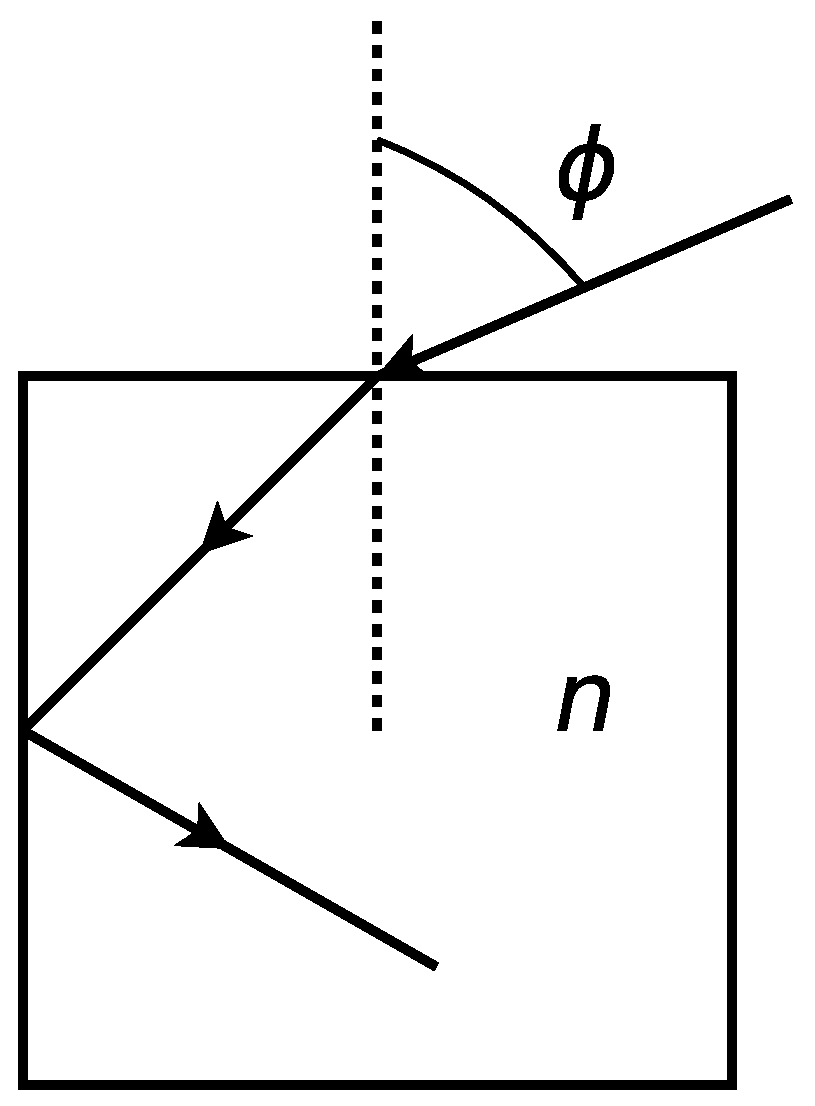
\includegraphics[width=\textwidth]{ej3-5}
\end{minipage}



\item
La fibra óptica es en esencia una hebra muy fina de un material de alto índice de refracción, e.g. cristal de silicio o plástico transparente.
Un revestimiento (\emph{cladding}) de menor índice logra, por reflexión total, que la luz que ingresa por un extremo al núcleo (\emph{core}) solo pueda salir por el otro.
\begin{figure}[ht]
	\centering{}\includegraphics[width=0.75\textwidth]{fibra}
\end{figure}
\begin{enumerate}
	\item Verifique que sufren reflexión total los rayos dentro del ángulo \(\alpha_A\) del cono de aceptación. 
	\[
		\sen{(\alpha_A)} = \frac{n_1}{n_o} \sqrt{1- \left( \frac{n_2}{n_1} \right)^2 }
	\]
	siendo \(n_0\), \(n_1\) y \(n_2\) índices de refracción del medio exterior, núcleo y recubrimiento.
	\item Como el cono de aceptación depende del índice que rodea a la fibra en el extremo de entrada, los fabricantes suelen informar para un sistema óptico (no solo fibras, también sistemas de lentes) la magnitud denominada \emph{apertura numérica} que se define como
	\[
		\text{AN} = n_0 \sen{(\alpha_A)},
	\]
	donde \(n_0\) es el índice de refracción del medio de donde proviene el haz que busca ingresarse en la fibra.

	Calcule la apertura numérica correspondiente a una fibra cuyo núcleo tiene un índice de refracción de \num{1.66} y el correspondiente a su recubrimiento es \num{1.4}.
	Para estos valores, ¿cuál es el ángulo de aceptación si la luz proviene del aire? ¿Y si proviene del agua?
	\item ¿Qué rango de valores debería tener el índice de refracción del recubrimiento de un núcleo cuyo índice es \num{1.66} para que todo rayo que incida desde el aire quede atrapado dentro de la fibra?
\end{enumerate}



\item Los índices de refracción de cierta clase de vidrio para el rojo y el violeta valen: $1.51$ y $1.53$; respectivamente.
Halle los ángulos límites de reflexión total para rayos que incidan en la superficie de separación vidrio-aire.
¿Qué ocurre si un rayo de luz blanca incide formando un ángulo de 41$^{\circ}$ sobre dicha superficie?
